\documentclass[11pt]{scrartcl}
\usepackage[noasy]{alan}
\usepackage{booktabs}
\usepackage{graphicx}
\usepackage{tikz}

\setkomafont{caption}{\small}
\setlist{itemsep=2pt}

\newcommand{\ket}[1]{\lvert #1\rangle}
\newcommand{\D}[2]{D^{#1}_{#2}}
\newcommand{\CZ}{\ensuremath{\mathrm{CZ}}}
\newcommand{\file}[1]{\texttt{\small #1}}

\title{Preparing Dicke States on Willow}
\subtitle{Four ideas behind our solution}
\author{Team Popeyes}
\date{DuQuantum $\times$ Google Quantum AI Challenge, Standard Track $\cdot$ October 25, 2026}

\begin{document}
\maketitle

\begin{abstract}
  Our function \file{create\_dicke\_state} builds a circuit that prepares a Dicke state exactly on
  Google's Willow chip. This note explains the four ideas that shaped it: (1) the judges' score
  rewards small, perfectly balanced cases far more than large ones; (2) W states can be spread out
  along a tree instead of a line; (3) for small cases a computer search finds much cheaper exact
  circuits than the textbook recipe; (4) where the circuit sits on the chip matters as much as what it
  is. We assume only vectors, $2\times2$ matrices, binomial coefficients and averages.

  All numbers come from \emph{simulation} with the calibrated error rates, energy decay
  ($T_1=68\,\mu$s~\cite{willow}), dephasing and readout errors. Nothing here has run on real hardware.
\end{abstract}

%% ---------------------------------------------------------------------------
\section{Background}

\subsection{Qubits and the Dicke state}

A \vocab{qubit} is a unit vector $a\ket0+b\ket1$ with $a^2+b^2=1$. Measuring it gives $0$ with
probability $a^2$ and $1$ with probability $b^2$. A state of $N$ qubits assigns an
\vocab{amplitude} $\psi_b$ to each of the $2^N$ bit strings $b$, and measuring all qubits gives
string $b$ with probability $\psi_b^2$. (Amplitudes may be complex in general, but every state in
this note is real.)

\begin{definition}[Dicke state]
  The \vocab{Dicke state} $\ket{\D Nn}$ is the equal superposition of every $N$-bit string with
  exactly $n$ ones. There are $K=\binom Nn$ such strings, each with amplitude $1/\sqrt K$. The case
  $n=1$ is called the \vocab{W state} $\ket{W_N}$.
\end{definition}

\begin{example}[$\D42$]
  $\ket{\D42}=\tfrac{1}{\sqrt6}\bigl(\ket{0011}+\ket{0101}+\ket{0110}+\ket{1001}+\ket{1010}+\ket{1100}\bigr)$.
  Measuring it gives each of these six strings with probability $1/6$.
\end{example}

The circuit must produce this vector \emph{exactly}, signs included, when there is no noise.

\subsection{Gates and their cost}

We may use any single-qubit gate, and one two-qubit gate, the \vocab{controlled-Z}
($\CZ$), which flips the sign of $\ket{11}$. A CZ only works between qubits that are physically
connected on the chip, and it fails about ten times as often as a single-qubit gate. So we measure a
circuit's cost mainly by its \vocab{CZ count}, and second by its \vocab{depth} (number of time
steps), because qubits also decay while they wait.

Two facts make the problem easier. First, flipping every bit turns $\ket{\D Nn}$ into
$\ket{\D N{N-n}}$, so we only build $n\le N/2$ and add a layer of $X$ gates when needed. Second,
swapping two qubits leaves a Dicke state unchanged, so any placement of a circuit on the chip is a
valid answer and qubit order never has to be fixed up.

%% ---------------------------------------------------------------------------
\section{Idea 1: the score rewards small, perfectly balanced cases}\label{sec:score}

\subsection{How the judges score}

For each test case $(N,n)$ the judges run our circuit $10^4$ times and measure every qubit, and
another $10^4$ times in a rotated basis that is sensitive to the signs of the amplitudes. The score
for the case is
\[
  S=\frac{1}{z+x}.
\]
\begin{itemize}
  \item The \textbf{$Z$ term} $z$ asks: \emph{is every valid string equally likely?} Shots with the
        wrong number of ones are thrown away, leaving a fraction $f$. The remaining counts are
        compared with a perfectly even split using Pearson's \vocab{chi-squared statistic}
        $\chi^2=\sum_b (\text{observed}_b-\text{expected})^2/\text{expected}$, and
        $z=\chi^2/(Kf)$.
  \item The \textbf{$X$ term} $x$ asks: \emph{are the signs right?} It compares averaged
        correlations in the rotated basis with their ideal values.
\end{itemize}
Small $z$ and $x$ mean a large score, and the total is the sum over all test cases.

\subsection{Why small \texorpdfstring{$K$}{K} is worth so much}

The score is the \emph{reciprocal} of a random number. If $z$ is usually around $1$ but sometimes
lands very close to $0$, then $S$ is usually around $1$ but sometimes enormous, and those rare
large values dominate the average.

\begin{fact}
  For a perfect state, $\chi^2$ behaves like a sum of $K-1$ squared standard normal variables (a
  $\chi^2_{K-1}$ distribution). With only one or two terms in the sum ($K=2$ or $3$), the sum lands
  near $0$ often enough that the average of $1/\chi^2$ is infinite. With more terms, it is
  $1/(K-3)$.
\end{fact}

So for $K=2,3$ only the $X$ term stops the expected score from blowing up. For a perfect state
($f=0.9$, $x=10^{-3}$):

\begin{center}\small
\begin{tabular}{lcccccc}
  \toprule
  $K$ & 2 & 3 & 4 & 6 & 10 & 20\\
  \midrule
  expected score $\EE[S]$ & 51.4 & 8.15 & 3.34 & 1.79 & 1.28 & 1.06\\
  \bottomrule
\end{tabular}
\end{center}

A single $K=2$ case (for example $W_2$) is worth about fifty large cases.

\subsection{Small imbalances destroy the bonus}

Suppose string $b$ appears with probability $(1+\delta_b)/K$ instead of $1/K$. Plugging this into
the chi-squared formula adds, on average,
\[
  \lambda=10^4 f\,\overline{\delta^2}
\]
to $\chi^2$, where $\overline{\delta^2}$ is the average of $\delta_b^2$. More importantly, $\chi^2$
can no longer land near $0$, so the lucky draws disappear. A 1\% imbalance gives $\lambda\approx0.9$
and drops the $K=2$ score from 51.4 to 33.3. A 3\% imbalance gives $\lambda\approx8$ and drops it to
1.3.

\begin{figure}[h]
  \centering
  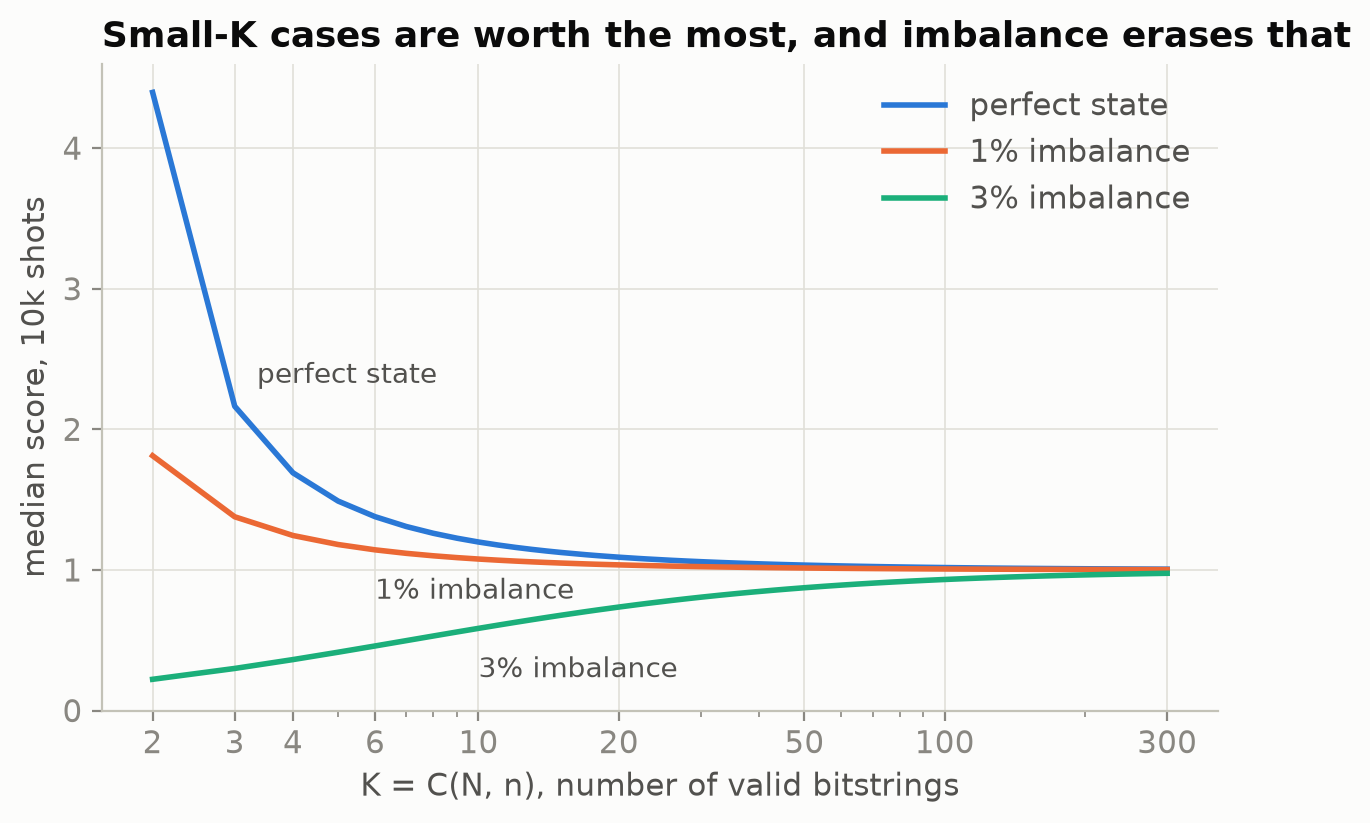
\includegraphics[width=0.6\linewidth]{figures/score_tail.png}
  \caption{Median single-run score against $K$ for a perfect state and for 1\% and 3\% imbalance.}
\end{figure}

\begin{remark}[Takeaway]
  Our priorities, in order: (1) always return a valid circuit, since any valid circuit scores above
  zero; (2) keep the small-$K$ cases balanced to within about 1\% and their signs accurate; (3) keep
  the fraction $f$ of valid shots high; (4) only then worry about large $N$. We may not fix a known
  bias by tilting the amplitudes, because the noiseless state must be exact. Balance has to come
  from the construction and from choosing good qubits.
\end{remark}

%% ---------------------------------------------------------------------------
\section{Idea 2: spread a W state along a tree, not a line}

A W state has a single excitation (a single ``1'') shared evenly among $N$ qubits. Think of it as
probability $1$ that must end up split into $N$ equal shares of $1/N$.

\begin{algorithm*}
  Choose a tree of connected qubits on the chip with root $r$. Start with $r$ in $\ket1$ and the
  rest in $\ket0$. In each round, every qubit $v$ that holds some probability passes to one child $c$
  exactly the share its subtree needs, $s(c)/N$, where $s(c)$ is the number of qubits under $c$
  (including $c$). This uses the two-qubit \vocab{transfer}
  \[
    \ket{10}\mapsto\sqrt{1-p}\,\ket{10}+\sqrt p\,\ket{01},\qquad \ket{00}\mapsto\ket{00},
  \]
  where $p$ is the fraction of $v$'s current share that moves to $c$.
\end{algorithm*}

\begin{example}[$W_4$ in two rounds]
  Take the four-qubit tree below, rooted at $r$.
  \begin{center}
  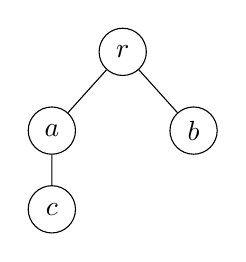
\begin{tikzpicture}[every node/.style={circle,draw,minimum size=6mm,inner sep=0pt},
      level distance=10mm, sibling distance=18mm]
    \node {$r$} child {node {$a$} child {node {$c$}}} child {node {$b$}};
  \end{tikzpicture}
  \end{center}
  Round 1: $r$ holds everything and gives half to $a$ (whose subtree has 2 of the 4 qubits).
  Round 2, both at once: $r$ gives half of its share to $b$, and $a$ gives half of its share to $c$.
  Every qubit now holds $1/4$. A line $r-a-c-b$ would need three rounds.
\end{example}

\textbf{Cost.} The very first transfer acts on the known state $\ket{10}$ and costs 1 CZ. Every
later transfer must handle both $\ket{00}$ and $\ket{10}$ correctly, and that needs 2 CZ. The total
is $1+2(N-2)=2N-3$ CZ, the same as a line, and an exhaustive search shows it is the minimum for
$W_3$ and $W_4$.

\textbf{Why a tree helps.} The tree does all transfers of a round at the same time, so it needs far
fewer rounds than a line, which needs $N-1$. For $W_{10}$ that means 15 time steps instead of 37,
and with idle noise the $X$ term drops from 0.0075 to 0.0042. The circuit also keeps exactly one
excitation in every branch at all times, so energy decay lowers every valid string equally and
creates no imbalance.

\begin{figure}[h]
  \centering
  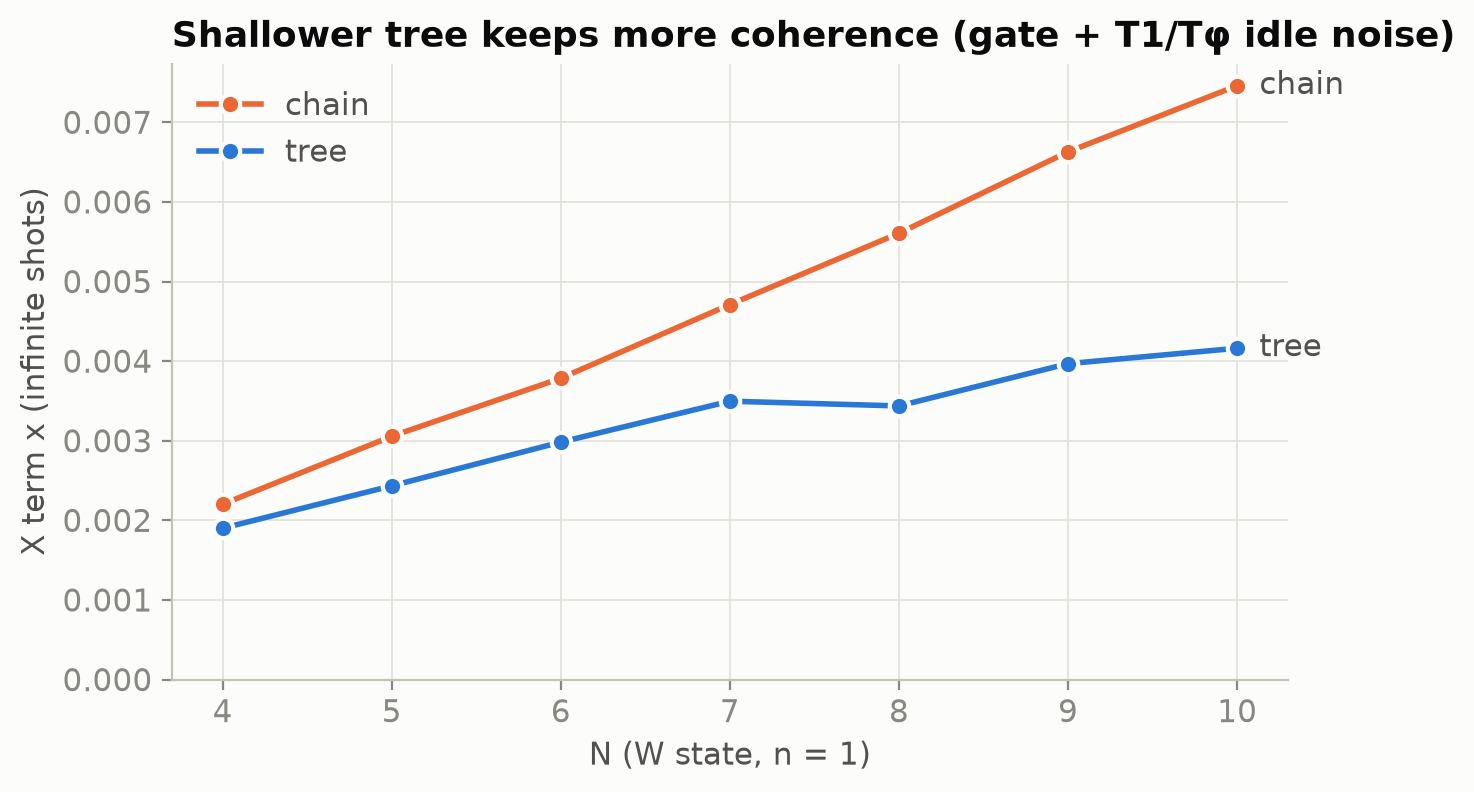
\includegraphics[width=0.6\linewidth]{figures/tree_vs_chain.png}
  \caption{$X$ term of $W_N$ under gate and idle noise: tree against line (chain).}
\end{figure}

%% ---------------------------------------------------------------------------
\section{Idea 3: let a computer search for exact circuits}\label{sec:synth}

The textbook construction of Bärtschi and Eidenbenz~\cite{be19} works for every $N$ and $n$, but it
uses gates between qubits that are not neighbours on the chip. Fixing that adds many CZs. For small
$N$ we instead let a computer find the circuit.

\textbf{The template.} Alternate layers of single-qubit rotations (each with its own angle) with
layers of CZ gates between neighbouring qubits. The output state $\ket{\psi(\theta)}$ depends on the
list of angles $\theta$.

\textbf{The search.} The circuit is exact when its output matches the Dicke state, so we minimize
the \vocab{infidelity}
\[
  \mathcal L(\theta)=1-\bigl(\text{overlap of }\ket{\psi(\theta)}\text{ with }\ket{\D Nn}\bigr)^2
\]
by gradient descent, until $\mathcal L<10^{-13}$ (exact to machine precision). Then we delete CZs
one at a time, re-optimize, and keep each deletion only if the circuit becomes exact again.

\begin{center}\small
\begin{tabular}{lcccccc}
  \toprule
  case & $\D42$ & $\D52$ & $\D63$ & $\D73$ & $\D83$ & $\D84$\\
  \midrule
  CZ, computer search & 5 & 10 & 15 & 25 & 31 & 27\\
  CZ, textbook (routed) & 21 & 35 & 80 & 98 & 123 & 162\\
  \bottomrule
\end{tabular}
\end{center}

The search takes minutes, so we run it once and store the angles in \file{main.py}. Often several
different angle sets are exact. We keep the one least sensitive to rotations that are slightly too
large, a systematic error our noise model does not include (for $\D52$ this cut the resulting
imbalance $\lambda$ from 50 to 9).

The search stops scaling at about $N=9$: overnight runs found exact circuits, but with more CZs than
the constructions we already had.

%% ---------------------------------------------------------------------------
\section{Idea 4: put the circuit on the best qubits}

Willow's qubits and connections differ a lot in quality, and because of permutation symmetry we are
free to place a circuit anywhere its shape fits. So we score every placement and keep the best one.

\textbf{The cost of a placement.} The fraction of good shots is roughly the probability that no
error happens anywhere, $f\approx\prod(1-e)$, over every gate, idle period and measurement. Taking
logarithms and using $\log(1-e)\approx-e$ for small $e$ turns this into a \emph{sum}: the cost of a
placement is the total error probability of all the gates, idling and readouts it uses. Sums are easy
to search over.

\textbf{Matching readout errors.} Measurement sometimes reads a 1 as a 0, and how often depends on
the qubit. A string whose ones sit on ``leaky'' qubits is read correctly less often, which creates
exactly the imbalance that Idea~1 says is so costly. A random choice of qubits gives about 0.6\%
imbalance from readout alone. Since we may not tilt the amplitudes to compensate, we add a penalty
for qubits whose readout errors differ, and prefer qubits that match.

\textbf{The smallest case.} For $W_2$ ($K=2$), which is worth the most, we simulate every possible
pair of connected qubits under the calibrated noise and keep the pair with the highest expected
score. This alone gains 9\% in expected score.

%% ---------------------------------------------------------------------------
\section{Putting it together}

The final \file{main.py} picks, for each $(N,n)$, the construction that scored best in simulation:
the tree for W states, the computer-found circuits for $N\le8$, and Bryan's independent
construction (a two-arm split that runs two smaller B-E circuits in parallel, written up in
\file{docs/bryan\_constructions.md}) for larger cases. Finally, consecutive single-qubit gates are
merged, and idle qubits get short pulse sequences (\vocab{dynamical decoupling}) that cancel slow
phase drift without changing the noiseless state.

\begin{center}\small
\begin{tabular}{lrlccc}
  \toprule
  case & $K$ & construction & CZ & $\EE[S]$ & \% of perfect\\
  \midrule
  $W_2$     &   2 & tree, best pair  &   2 $\to$ 1  & 54.3 $\to$ 65.6 & 96\\
  $W_3$     &   3 & tree             &   4 $\to$ 3  &  7.45 $\to$ 7.97 & 97\\
  $\D42$    &   6 & computer search  &  21 $\to$ 5  &  1.55 $\to$ 1.85 & 95\\
  $\D63$    &  20 & computer search  &  80 $\to$ 15 &  0.54 $\to$ 1.03 & 88\\
  $\D84$    &  70 & computer search  & 162 $\to$ 27 &  0.24 $\to$ 0.80 & 77\\
  $\D{10}5$ & 252 & Bryan's          & 324 $\to$ 85 &  0.12 $\to$ 0.39 & 39\\
  \bottomrule
\end{tabular}
\end{center}

Arrows read ``first-day baseline $\to$ final''. The last column compares our expected score with
that of a perfect, noiseless state. Over all 25 cases with $N\le10$ our expected total is 102.0, out
of 218.7 for a perfect state. $W_2$ and $W_3$ alone account for 73.5 of our total, which is exactly
the concentration that Idea~1 predicted and that drove the whole design. The full table is in
\file{ARCHITECTURE.md}.

\subsection*{What we learned}

\begin{itemize}
  \item \textbf{Read the scoring rule before optimizing.} The score is dominated by a handful of
        small cases, and for those, balance matters more than raw gate count.
  \item \textbf{Cheap exact circuits come from search, not from textbooks,} but only up to about
        nine qubits.
  \item \textbf{Hardware quality varies,} so choosing qubits is an optimization problem of its own.
  \item \textbf{Limits.} Our simulator ignores crosstalk, slow drift and systematic rotation errors,
        so real hardware will score lower than these numbers.
\end{itemize}

\bibliographystyle{abbrv}
\bibliography{refs}

\end{document}
